\documentclass{article}
\usepackage{lmodern}            % Smoothly scaling font.
\usepackage[                    % Set the default font size.
fontsize=24,
]{fontsize}
\renewcommand{\familydefault}{\sfdefault}
\usepackage[
% - HP DesignJet Z5200 printer in the Chemical Engineering department
%   has a 44" roll width (1118 mm).
% - The FacultyHack @ Science Gateways 2025 conference allows 30"x45"
% - Therefore, crop the poster to 44in height i.e. 30"x44"
paperwidth=30in,
paperheight=44in,
margin=0.5cm,
head=2.47in,
foot=1.59in,
includeheadfoot,
%showframe,
]{geometry}
\usepackage{fancyhdr}
\title{GPUs for massively parallel mechanistic modeling}
\pagestyle{fancy}
\renewcommand{\headrulewidth}{0pt}
\renewcommand{\footrulewidth}{0pt}
\fancyhead[L]{%
  \begin{tikzpicture}[%
    background rectangle/.style = {
      fill = fh-blue,
    },
    show background rectangle,
    tight background,
    scale = 1]
    \node (ref) [
    minimum width = \paperwidth - 1cm,
    minimum height = 2.47in] {};
    \node at (ref.north west) [anchor = north west, name = fh] {%
      
\includegraphics[height=2.47in]{fh.png}};
    \node at (ref.south east) [%
    anchor = south east, %
    name = nsf-text,
    text = fh-gold,
    scale = 0.5,
    inner sep = 6pt,
    text width = width("under award number 2231406"),
    align = center] {%
      SGX3 is funded by the \mbox{National Science Foundation} %
      under award number 2231406};
    \path let
    \p1 = (ref.north),
    \p2 = (nsf-text.north),
    \n1 = {(\y1 - \y2) - 4pt} in
    node at (nsf-text.north) [anchor = south, name = nsf, yshift = -2pt] {%
      
\includegraphics[height=\n1]{nsf.png}};
    \node at (fh.east) [%
    anchor = west,
    text = fh-gold,
    scale = 3,
    text width = width("GPUs for massively parallel")] {%
      GPUs for massively parallel mechanistic modeling%
    };
  \end{tikzpicture}%
}
\fancyhead[C,R]{}
\fancyfoot[L]{%
  \begin{tikzpicture}[%
    background rectangle/.style = {
      fill = fh-blue,
      inner sep = 0pt,
    },
    show background rectangle,
    tight background,
    scale = 1]
    \pgfdeclarelayer{foreground}
    \pgfsetlayers{background,main,foreground}
    \begin{pgfonlayer}{foreground}
    \node (ref) [
    inner sep = 0,
    minimum width = 30in - 1cm,
    minimum height = 1.59in] {};
    \node (sgx3) at ([xshift=0.5cm]ref.west) [anchor = west] {%
      
\includegraphics[height=0.85in]{sgx3.png}};
    \node (ornl) at (sgx3.east) [anchor = west] {%
      
\includegraphics[height=1.04in]{ornl.png}};
    \node (omnibond) at (ornl.east) [anchor = west] {%
      
\includegraphics[height=0.87in]{omnibond.jpg}};
    \node (tacc) at (omnibond.east) [anchor = west] {%
      
\includegraphics[height=0.87in]{tacc.png}};
    \node (qr-code) at (ref.east) [anchor = east, outer sep = 0.25cm] {%
      
\includegraphics[height=1.32in]{qr-code.png}};
    \node at (qr-code.west) [anchor = east, text = fh-gold, scale = 1.6] {%
      \textbf{Event Site:} %
      \url{https://hackhpc.github.io/facultyhack-gateways25}
      };
    \end{pgfonlayer}
    \begin{pgfonlayer}{main}
      \node [
      inner sep = 0pt, fit = (sgx3) (ornl) (omnibond) (tacc), fill = white] {};
    \end{pgfonlayer}
  \end{tikzpicture}%
}
\fancyfoot[C]{}

\usepackage{graphicx}
\graphicspath{{img/}}

\usepackage{multicol}
\setlength\columnseprule{0pt}
\setlength{\columnsep}{2.5pc}

\usepackage{tikz}
\usepackage{tikz}
\tikzset{
  every node/.style = {
    inner sep = 0pt,
    outer sep = 0pt
  }
}
\usetikzlibrary{
arrows.meta,
backgrounds,
calc,
decorations.markings,
decorations.pathmorphing,
decorations.text,
fit,
mindmap,
tikzmark
}

\usepackage{soul}

\usepackage{amssymb}            % \blacksquare
\usepackage{amsmath}            % \text

\usepackage{tabularx}
\newcolumntype{C}{>{\centering\arraybackslash}X}
\newcolumntype{R}{>{\raggedleft\arraybackslash}X}
% Vertically center within row https://tex.stackexchange.com/a/343329
\renewcommand\tabularxcolumn[1]{m{#1}}
\usepackage{booktabs}
\usepackage{multirow}

\usepackage[
abbreviate=true,
bibencoding=utf8,
minnames=2,
maxbibnames=99,
sorting=none,
style=vancouver,
citestyle=numeric-comp
]{biblatex}
% The vancouver citation style is based on NLM per
% https://tex.stackexchange.com/a/371433
\addbibresource{references.bib}
\renewcommand*{\bibfont}{\footnotesize\selectfont}

\usepackage[
table
]{xcolor}
\definecolor{fh-blue-lighter}{HTML}{EBEFF7}
\definecolor{fh-blue-darker}{HTML}{D4DEED}
\definecolor{fh-blue}{RGB}{0,89,157}
\definecolor{fh-gold}{HTML}{F7E8C9}

\usepackage{tcolorbox}
\newcommand{\sectionbox}[1]{%
  \begin{tcolorbox}[sharp corners,boxrule=0pt,top=15pt,colback=fh-blue,coltext=fh-gold]%
    \section*{#1\vphantom{Yy}}%
  \end{tcolorbox}%
}

\begin{document}

\begin{multicols}{2}

  \sectionbox{Introduction}%
  \noindent
  Graphical Processing Units (GPUs) %
  are integrated into the core architecture %
  of the world's fastest supercomputers %
  that solve the most computationally difficult, %
  mechanistic scientific problems.
  %
  An 8~year, \$1.8~billion effort %
  called the Exascale Computing Project (ECP) %
  involving 2,800 scientists and engineers %
  recently finished modernizing %
  the underlying scientific numerical software %
  to efficiently use this new generation of machines.
  \smallskip

  \noindent
  Computing facilities grant access at no cost %
  to these GPU-accelerated%
  \supercite{%
    carter_2014,%
    beckingsale_2019,%
    reinders_2023%
  } machines %
  only to research software engineers and scientists who demonstrate that %
  their computations scale %
  to efficiently use multiple GPUs across many computer servers / nodes.
  %
  Therefore, %
  it is imperative to teach %
  the data parallel software development skills, %
  appropriate domain science methods, and %
  sustainable software practices %
  to enable large scale, GPU-centric computational research.
  \smallskip

  \noindent
  Discussion and feedback on this poster from the community %
  can help make this course a success and %
  support similar hands-on learning and teaching endeavors.
  \smallskip

  \noindent
  \begin{minipage}[c]{.36\linewidth}
    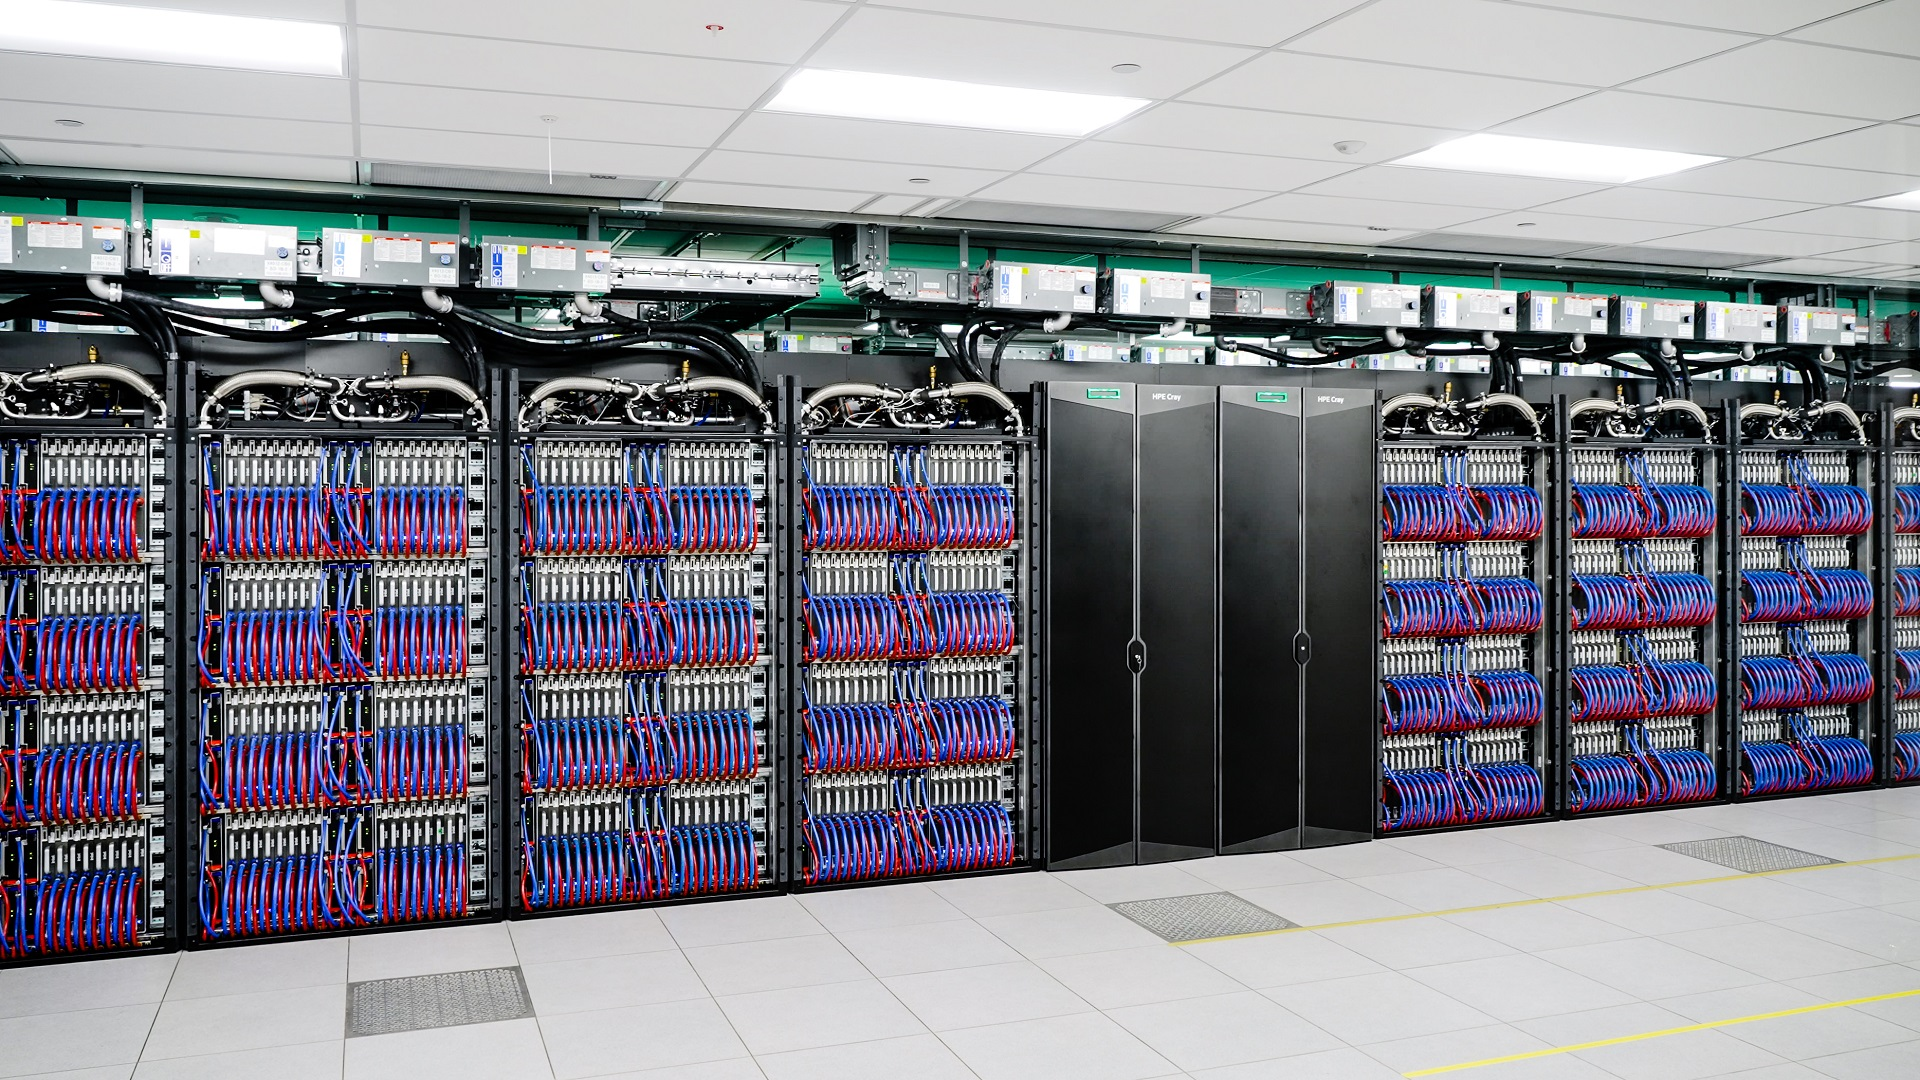
\includegraphics[width=\linewidth]{1920x1080-Aurora hero image.jpg}
  \end{minipage}
  \begin{minipage}[c]{.62\linewidth}
    \textbf{Modern supercomputers use GPU architectures.}
    %
    Left photo is the Aurora supercomputer at Argonne National Laboratory %
    that is ranked 3\textsuperscript{rd} in the Top 500 List of June 2025 %
    and one of three US exascale supercomputers.
    %
    Germany recently launched their first exascale supercomputer, JUPITER, %
    and China may have as many as 10 exascale supercomputers %
    by the end of this year\supercite{dongarra_2023} %
    but stopped submitting data to the Top 500 List %
    after US GPU embargoes.
  \end{minipage}
  \vspace{\baselineskip}

  \subsection*{\textcolor{fh-blue}{Target Course Description}}

  {
    \rowcolors{1}{fh-blue-lighter}{fh-blue-darker}
    \begin{tabularx}{\linewidth}{>{\bfseries}r X}
      \toprule
      Course Name:
      & GPUs for massively parallel mechanistic modeling\\
      Course Number:
      & TBA\\
      Department:
      & Chemical Engineering\\
      Anticipated Enrollment:
      & 12\\
      Prerequisites:
      & fluent with at least one %
      procedural programming language\\
      Key Content:
      & performance optimization, %
      software development, %
      domain science methods, %
      capstone project\\
      Description:
      & This course trains graduate researchers %
      with ECP-level skills in high performance computing (HPC), %
      using research software engineer (RSE) rigor, %
      and HPC-relevant domain scientific methods.\\
      Project Repo:
      & \small \url{https://github.com/omsai/facultyhack-gateways25-nanda}\\
      \bottomrule
    \end{tabularx}
  }

  \subsection*{\textcolor{fh-blue}{Goals}}
  \begin{itemize}
  \item Setup student \ul{JetStream2 VM} for homework and capstone projects.
  \item Add students to my \ul{ACCESS group} for cluster runs and %
    help them get their own ACCESS allocation.
  \item Teach all C++ classroom exercises inside a \ul{web IDE}. 
  \item Train students to \ul{package their project}.
  \end{itemize}

  \sectionbox{Initial Course Syllabus}%
  \noindent
    \textbf{High-level comparison of topics.}
        %
        Comparison of this course with the %
        2024 Argonne Training Program on Extreme-Scale Computing (ATPESC'24) %
        and the 2025 Lawrence Livermore National Laboratory %
        High Performance Computing Innovation Center (HPC-IC'25) %
        tutorial series.
        \medskip

    \noindent
    \begin{tabularx}{\linewidth}{%
      >{\hsize=.15\hsize\linewidth=\hsize}X %
      >{\hsize=.34\hsize\linewidth=\hsize}R %
      >{\hsize=.16\hsize\linewidth=\hsize}C %
      >{\hsize=.16\hsize\linewidth=\hsize}C %
      >{\hsize=.16\hsize\linewidth=\hsize}C}
      \toprule
      \textbf{Category}
      & \textbf{Topic}
      & \textbf{This Course} & \textbf{ATPESC'24} & \textbf{HPC-IC'25}\\
      \midrule
      \multirow{4}{\hsize}{Performance optimization}
      & Within node
      & \checkmark & \checkmark & $\times$\\
      & Multi-node
      & \checkmark & \checkmark & \checkmark\\
      & GPU performance portability
      & \checkmark & \checkmark & \checkmark\\
      & Performance tuning
      & \checkmark & \checkmark & \checkmark\\
      \midrule
      \multirow{7}{\hsize}{Software development}
      & Unit testing
      & \checkmark & \checkmark & $\times$\\
      & Performance testing
      & \checkmark & \checkmark & \checkmark\\
      & Continuous integration
      & \checkmark & $\times$ & \checkmark\\
      & Checkpointing
      & \checkmark & $\times$ & \checkmark\\
      & Parallel debugging
      & \checkmark & \checkmark & $\times$\\
      & Code peer review
      & \checkmark & $\times$ & $\times$\\
      & Reproducibility
      & \checkmark & \checkmark & \checkmark\\
      \midrule
      \multirow{-0.5}{\hsize}{Domain science methods}
      & \mbox{Gradient-free optimization of\ldots{}} %
        \mbox{\ldots{}scientific model parameters}
      & \checkmark & $\times$ & $\times$\\
      & Mechanistic multiscale modeling
      & \checkmark & $\times$ & $\times$\\
      & Coupling AI, cloud, data science
      & \checkmark & $\times$ & \checkmark\\
      \midrule
      \multirow{2}{\hsize}{Sysadmin}
      & Cluster launch
      & \checkmark & $\times$ & \checkmark\\
      & Cluster profiling
      & \checkmark & \checkmark & \checkmark\\
      \bottomrule
    \end{tabularx}
    \bigskip

  \sectionbox{Modified Course Syllabus}

    \bigskip
    \begin{minipage}[c]{.27\linewidth}
      \textbf{Course topics.}
          %
          The topics covered in this course %
          are organized into the categories of the %
          \textcolor{red!80!black}{$\blacksquare$}~capstone project,
          \textcolor{orange!90!black}{$\blacksquare$}~performance optimization, %
          \textcolor{blue!80!black}{$\blacksquare$}~software development, %
          \textcolor{green!50!black}{$\blacksquare$}~domain science methods, and %
          \textcolor{black!60}{$\blacksquare$}~cluster administration.
          %
          Each leaf node more-or-less corresponds to %
          a single week of semester classroom sessions.
    \end{minipage}
    %\hfill
    \begin{minipage}[c]{.73\linewidth}
      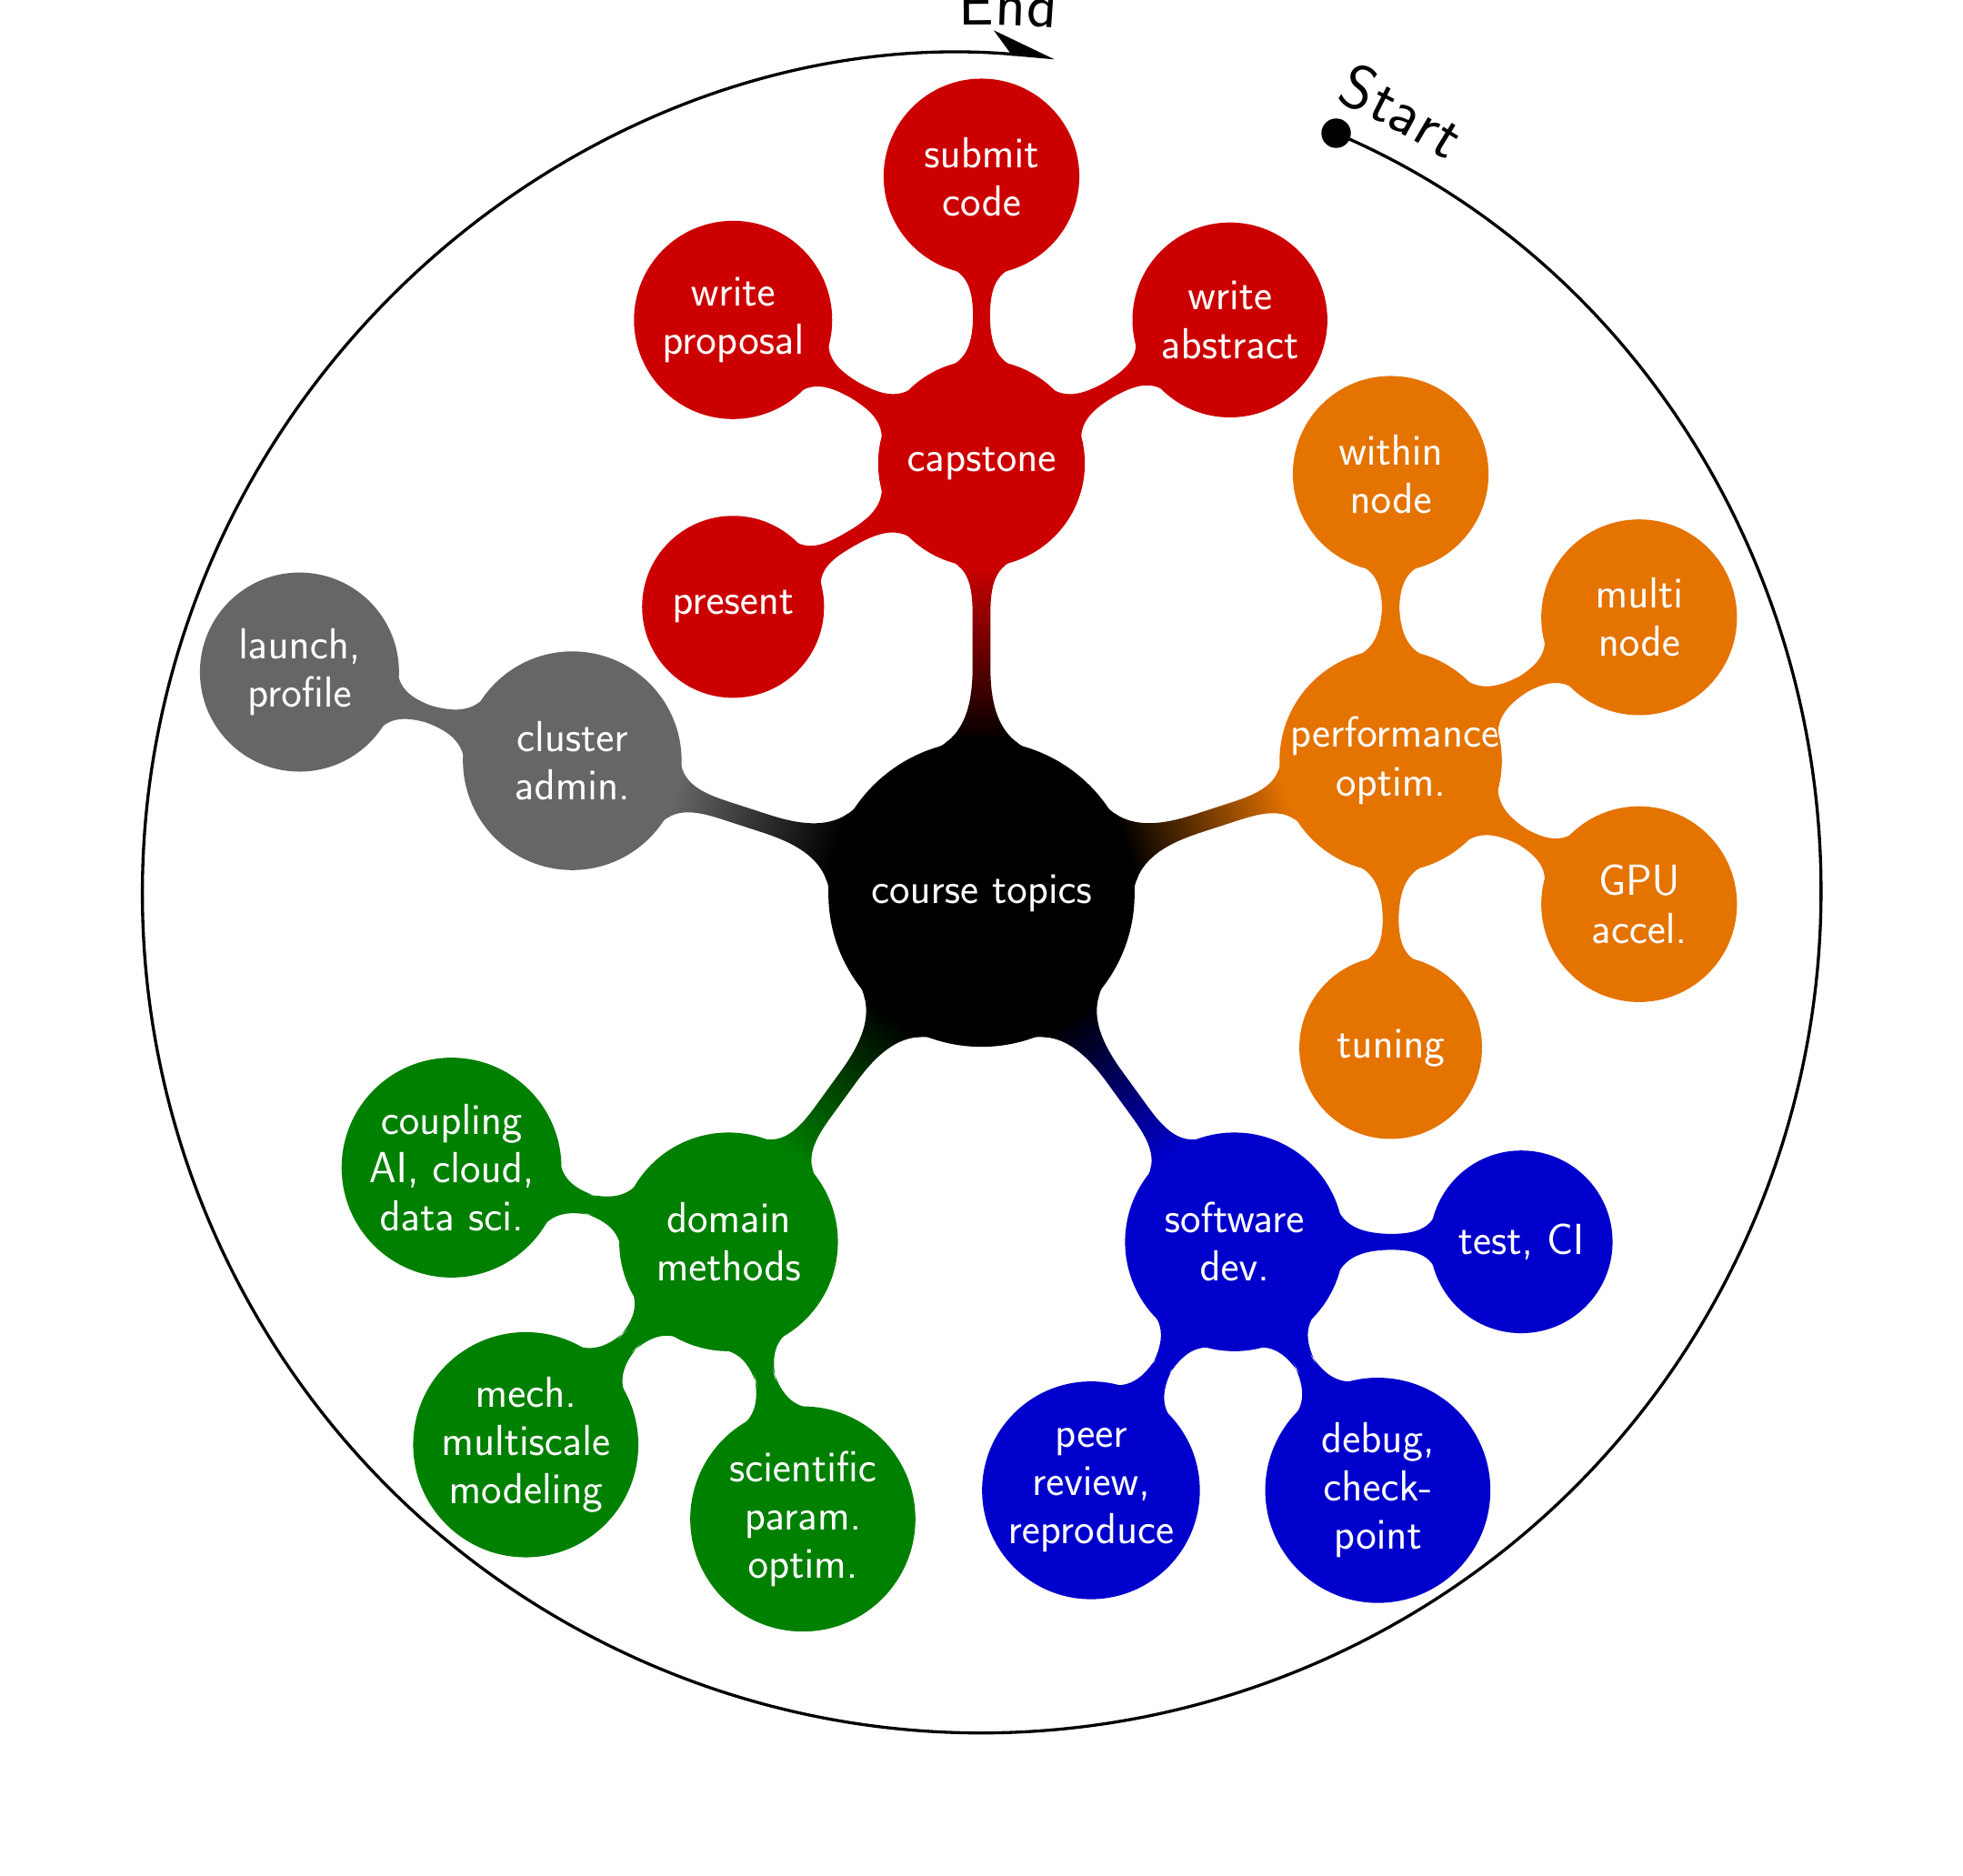
\begin{tikzpicture}[
        scale = 0.95,
        root concept/.style={
          text width = 120pt,
        },
        level 1 concept/.style={
          text width = 80pt,
          level distance = 180,
        },
        level 2 concept/.append style={
          text width = 70pt,
          level distance = 120,
        },
        every concept/.append style={
          font = \scriptsize,
        },
        mindmap,
        ]
        \path
        node [concept, concept color=black, text=white, name=node-concept]
        {course topics}
        child [grow=90, concept color=red!80!black, text=white] {
          node [concept] {capstone}
          [clockwise from=210]
          child { node [concept] {present} }
          child { node [concept] {write proposal} }
          child { node [concept] {submit code} }
          child { node [concept] {write abstract} }
        }
        child [grow=18, concept color=orange!90!black, text=white] {
          node [concept] {performance optim.}
          [clockwise from=90]
          child { node [concept] {within node} }
          child { node [concept] {multi node} }
          child { node [concept] {GPU accel.} }
          child { node [concept] {tuning} }
        }
        child [grow=306, concept color=blue!80!black, text=white] {
          node [concept] {software dev.}
          [clockwise from=0]
          child { node [concept] {test, CI} }
          child { node [concept] {debug, checkpoint} }
          child { node [concept] {peer review, reproduce} }
        }
        child [grow=234, concept color=green!50!black, text=white] {
          node [concept] {domain methods}
          [clockwise from=285]
          child { node [concept] {scientific param. optim.} }
          child { node [concept] {mech. multiscale modeling} }
          child { node [concept] {coupling AI,~cloud, data sci.} }
        }
        child [grow=162, concept color=black!60, text=white] {
          node [concept] {cluster admin.}
          [clockwise from=162]
          child { node [concept] {launch, profile} }
        };
        \draw [%
        very thick,
        {Circle[length=0.5em]-Stealth[harpoon,length=1em]},
        postaction={
          decorate,
          decoration={
            text align={left},
            raise={0.5em},
            text along path,
            text={Start}
          }
        },
        postaction={
          decorate,
          decoration={
            text align={right},
            raise={0.5em},
            text along path,
            text={End}
          }
        }]
        ([shift=(66:15em)]node-concept) arc (66:-275:15em);
      \end{tikzpicture}
    \end{minipage}

  \sectionbox{Mentors Suggestions}%
  \begin{multicols}{2}
    \begin{enumerate}
    \item \ul{Added network communication exercises} %
      using the LAMMPS exercise developed at Temple University.
    \item \ul{Added profiling exercises} %
      from Cornell University %
      and the University of Michigan.
    \item \ul{Chose a checkpointing library} %
      written in C/C++ %
      both to teach in the course %
      and to recommend for student capstone projects.
    \item Trainees will \ul{write C/C++ code using VS Code} %
      with SSH tunnels to JetStream2 virtual machines %
      with a fallback of OpenVSCode Server web interface %
      for classroom instruction.
    \item \ul{Added an AI policy} %
      that requires a bibliography %
      citing AI service names with versions, prompts, and output.
    \item Moved non-capstone homework assignments to %
      \ul{classroom hands-on to avoid over-reliance on AI support} %
      while trainees are still developing expertise.
    \item \ul{Increased accessibility} %
      to less experienced C/C++ programmers %
      by recommending self-guided, open access textbooks %
      from \emph{The Art of HPC: Volume 3}.
    \item \ul{Added objective of numerical correctness} %
      but limited goal to unit tests, performance test, and CI %
      instead of considering formal methods.
    \item The target audience is now \ul{graduate students} %
      with existing projects or pilot projects.
    \item \ul{Consolidated course topics} %
      to allow for more focus on domain science methods %
      in keeping with the course title.
    \end{enumerate}
  \end{multicols}

  \sectionbox{Science Gateways Resources Used}%
  \begin{tikzpicture}
    \node (ref) [minimum width = \linewidth] {};

    \node (jetstream) at (ref.north west) [anchor = north west] {%
      
\includegraphics[width=.2\linewidth]{jetstream2-head-logo.pdf}};
    \node (jetstream-text) at (jetstream.north east) [%
    anchor = north west, text width = .78\linewidth] {%
    \textbf{Non-virtual multi-GPU A100 nodes (g3.2xl)}
    \begin{itemize}
    \item Shared between small groups of 4 students.
    \item For early project development and exercises.
    \item A100 supports 64-bit floating point operations %
      for capstone projects that may require it.
    \item Efficient multi-GPU use is a course objective.
    \item g3.2xl is the multi-GPU A100 with the most availability.
    \end{itemize}
    };

    \node (access) at (jetstream.west |- jetstream-text.south) [%
    anchor = north west, yshift = -\baselineskip] {%
      
\includegraphics[width=.2\linewidth]{access-logo.pdf}};
    \node (access-text) at (access.north east) [%
    anchor = north west, text width = .78\linewidth] {%
    \textbf{Bridges-2 GPU HPC Allocation}
    \begin{itemize}
    \item For cluster exercises and scaling.
    \item Interactive nodes with backfill scheduling and short walltime %
    for the classroom use.
  \item Trainees are encouraged %
    to apply for their own ACCESS CI allocations %
    to continue their work %
    after leaving the instructor's ACCESS CI group.
    \end{itemize}
    };

    \node (hpcc) at (access.west |- access-text.south) [%
    anchor = north west, yshift = -\baselineskip] {%
      
\includegraphics[width=.2\linewidth]{hpc-carpentry.pdf}};
    \node (hpcc-text) at (hpcc.north east) [%
    anchor = north west, text width = .78\linewidth] {%
    \textbf{HPC introduction and reproducible workflows}
    \begin{itemize}
    \item Self-paced introduction to key concepts of the  HPC environment.
    \item Supplementary reading for %
      capstone project reproducible workflows %
      for coupling AI, cloud, and data science tools.
    \end{itemize}
    };

    \node (gha) at (hpcc.west |- hpcc-text.south) [%
    anchor = north west, yshift = -\baselineskip] {%
      
\includegraphics[width=.1\linewidth]{github-mark.pdf}%
      
\includegraphics[width=.1\linewidth]{actions-icon-actions.pdf}};
    \node (gha-text) at (gha.north east) [%
    anchor = north west, text width = .78\linewidth] {%
    \textbf{Trainee GitHub repositories for assignments and capstone projects}
    \begin{itemize}
    \item Projects in private git repositories shared with the instructor.
    \item Assignments partially checked using GitHub actions.
    \item Progress on capstone projects will be monitored from git repositories.
    \end{itemize}
    };
  \end{tikzpicture}

  \sectionbox{Expansions}%
  \begin{multicols}{2}
    \begin{enumerate}
    \item Accommodate \ul{undergraduate students} %
      with more structure, %
      shorter exercises, %
      and allow them to choose from a set of smaller capstone projects.
    \item For the last ``fun'' topic before final presentations %
      \ul{launch the cluster using Raspberry Pis}, %
      networking hardware, and network storage %
      for a more memorable hands-on lesson.
    \item Develop an \ul{time-saving exercise for model comparison} %
      to demonstrate the usefulness %
      of detailed benchmarking and analysis tools %
      \ul{to rapidly iterating model development}.
    \item Create \ul{interactive trivial exercises in a web page} %
      to encourage trainee progress with %
      a live updating grading rubric %
      and suggestions to correct common errors.
    \item \ul{Compartmentalize topics %
      into the 2-day workshop format} %
      to be taught at the Pittsburgh Supercomputing Center (PSC).
    \end{enumerate}
  \end{multicols}

  \sectionbox{References}
  {
    % Recalculate \columnsep instead of using the large \columnsep
    % from the main document.
    \setlength{\columnsep}{1.5pc}
    \begin{multicols}{2}
      \printbibliography[heading=none]{}
    \end{multicols}
  }

  \sectionbox{Authors}%
  {
    \setlength{\parindent}{5em}

    \textbf{\textcolor{fh-blue}{\tikzmark{pn}Nanda, Pariksheet}}

    Role: Faculty Participant

    University of Pittsburgh

    pan79@pitt.edu
    \vspace{\baselineskip}

    \textbf{\textcolor{fh-blue}{\tikzmark{em}MacCarthy, Elijah}}

    Role: Community Mentor

    Oak Ridge National Laboratory

    maccarthyea@ornl.gov
  }
  \begin{tikzpicture}[%
    remember picture,
    overlay]
    \node at (pic cs:pn) [%
    anchor = north east,
    yshift = \baselineskip] {%
    \includegraphics[%
    keepaspectratio,
    width=10em,
    height=5em,
    clip,
    trim={55 85 50 35}]{%
        pariksheet.png}};

    \node at (pic cs:em) [%
    anchor = north east,
    yshift = \baselineskip] {%
    \includegraphics[%
    keepaspectratio,
    width=10em,
    height=5em,
    clip,
    trim={20 80 60 5}]{%
        elijah.jpg}};
  \end{tikzpicture}

\end{multicols}

\end{document}
